%Summer 2020 MT2
% Neelesh Ramachandran <neelesh.r@berkeley.edu>
\qns{Resist the Power!}

\begin{enumerate}[series = qn]
\item (4 points) You are given a resistive slab with resistivity $5.7\si{\ohm\cdot\centi\meter}$ and dimensions $0.9\si{\centi\meter}$, $2.7\si{\centi\meter}$, and $7.7\si{\centi\meter}$ as denoted on the figure below. The dimensions and the resistivity of the slab remain the same throughout the rest of the problem. % $0.9 < 2.7 < 7.7$. 

\begin{figure}[h]
	\begin{center}
		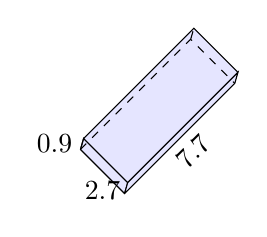
\begin{tikzpicture}[scale=1, x={(0.14cm,-0.14cm)},y={(0.04cm,0.14cm)},z={(-1.4cm,-1.4cm)}]
		\pgfmathsetmacro{\x}{4}
		\pgfmathsetmacro{\y}{1}
		\pgfmathsetmacro{\z}{1}
		\path (0,0,\y) coordinate (A) (\x,0,\y) coordinate (B) (\x,0,0) coordinate (C) (0,0,0)
		coordinate (D) (0,\z,\y) coordinate (E) (\x,\z,\y) coordinate (F) (\x,\z,0) coordinate (G)
		(0,\z,0) coordinate (H);
		\draw[fill=blue!10] (A)--(E)--(F)--(B);
		\draw[fill=blue!10] (A)-- node[below]{$2.7$} (B)-- node[below,sloped]{$7.7$} (C)--(G)--(F)--(B) (A)-- node[left]{$0.9$}(E)--(F)--(G)--(H)--(E);
		\draw [dashed,black] (A)--(D)--(C) (D)--(H);
		\end{tikzpicture}
	\end{center}
\end{figure}


Suppose we connect opposite faces of the slab to a voltage source so that current can flow through it. Notice that there are 3 possible configurations we can have for this slab, leading to 3 possible directions in which the current can flow (drawn in the answer choices below). Which direction will lead to the \textbf{highest} current flow $I$ assuming we use the same valued voltage source all three times? 
\\
Assume the resistivity is the same throughout the slab and does not vary with respect to the direction of current flow.

\begin{multicols}{2}
  \begin{enumerate}
  	\setlength\itemsep{2cm}
\item Parallel to $0.9$ (current goes through $2.7$, $7.7$ face): \\
\begin{minipage}{0.5\linewidth}
    \begin{center}
        \begin{tikzpicture}[scale=2, x={(0.14cm,-0.14cm)},y={(0.04cm,0.14cm)},z={(-1.4cm,-1.4cm)}]
            \pgfmathsetmacro{\x}{4}
            \pgfmathsetmacro{\y}{1}
            \pgfmathsetmacro{\z}{1}
            \path (0,0,\y) coordinate (A) (\x,0,\y) coordinate (B) (\x,0,0) coordinate (C) (0,0,0)
            coordinate (D) (0,\z,\y) coordinate (E) (\x,\z,\y) coordinate (F) (\x,\z,0) coordinate (G)
            (0,\z,0) coordinate (H);
            \draw[fill=blue!10] (A)--(E)--(F)--(B);
            \draw[fill=blue!10] (A)-- node[below]{$2.7$} (B)-- node[below,sloped]{$7.7$} (C)--(G)--(F)--(B) (A)-- node[left]{$0.9$}(E)--(F)--(G)--(H)--(E);
            \draw [dashed,black] (A)--(D)--(C) (D)--(H);
            \draw[-*, dashed, red, thick] (1.5, -3.3, 0.5)-- (-0.3, -3.3, 0.3);
            \draw[->, red, thick] (-0.3, -3.3, 0.3)-- (-2.1, -3.3, 0.1);
            \node[red] at (-2.5, -3.4, 0.1) {\fontsize{8}{7} $I$};
        \end{tikzpicture}
    \end{center}
  \end{minipage}

\item Parallel to $7.7$ (current goes through $0.9$, $2.7$ face): \\
\begin{minipage}{0.5\linewidth}
      \begin{center}
          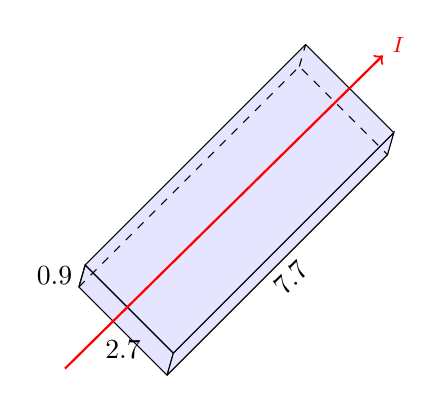
\begin{tikzpicture}[scale=2, x={(0.14cm,-0.14cm)},y={(0.04cm,0.14cm)},z={(-1.4cm,-1.4cm)}]
              \pgfmathsetmacro{\x}{4}
              \pgfmathsetmacro{\y}{1}
              \pgfmathsetmacro{\z}{1}
              \path (0,0,\y) coordinate (A) (\x,0,\y) coordinate (B) (\x,0,0) coordinate (C) (0,0,0)
              coordinate (D) (0,\z,\y) coordinate (E) (\x,\z,\y) coordinate (F) (\x,\z,0) coordinate (G)
              (0,\z,0) coordinate (H);
              \draw[fill=blue!10] (A)--(E)--(F)--(B);
              \draw[fill=blue!10] (A)-- node[below]{$2.7$} (B)-- node[below,sloped]{$7.7$} (C)--(G)--(F)--(B) (A)-- node[left]{$0.9$}(E)--(F)--(G)--(H)--(E);
              \draw [dashed,black] (A)--(D)--(C) (D)--(H);
              \draw[->, red, thick] (2, 1.3, 1.3)-- (2, 1, -0.15);
              \node[red] at (2, 1, -0.2) {\fontsize{8}{7} $I$};
          \end{tikzpicture}
      \end{center}
\end{minipage}

\item Parallel to $2.7$ (current goes through $0.9$, $7.7$ face): \\ 
\begin{minipage}{0.5\linewidth}
      \begin{center}
          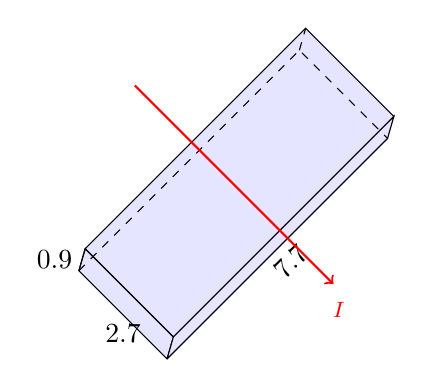
\begin{tikzpicture}[scale=2, x={(0.14cm,-0.14cm)},y={(0.04cm,0.14cm)},z={(-1.4cm,-1.4cm)}]
            \pgfmathsetmacro{\x}{4}
            \pgfmathsetmacro{\y}{1}
            \pgfmathsetmacro{\z}{1}
            \path (0,0,\y) coordinate (A) (\x,0,\y) coordinate (B) (\x,0,0) coordinate (C) (0,0,0)
            coordinate (D) (0,\z,\y) coordinate (E) (\x,\z,\y) coordinate (F) (\x,\z,0) coordinate (G)
            (0,\z,0) coordinate (H);
            \draw[fill=blue!10] (A)--(E)--(F)--(B);
            \draw[fill=blue!10] (A)-- node[below]{$2.7$} (B)-- node[below,sloped]{$7.7$} (C)--(G)--(F)--(B) (A)-- node[left]{$0.9$}(E)--(F)--(G)--(H)--(E);
            \draw [dashed,black] (A)--(D)--(C) (D)--(H);
            \draw[->, red, thick] (-1, 5.4, 0.8)-- (8, 5.4, 0.8);
            \node[red] at (8.3, 4.5, 0.8) {\fontsize{8}{7} $I$};
          \end{tikzpicture}
      \end{center}
\end{minipage}

\item Choices (A) and (C) are tied for the maximum current flow.
\item The direction doesn't matter; the resistor is physically the same, so the current will be the same.
  \end{enumerate}
  
  \end{multicols}
  
\ans{A}

\ans{For a given supply voltage from a voltage source, the most current will flow when the resistance of the slab is smallest. We apply the geometrical resistance formula, $R=\frac{\rho L}{A}$. To maximize current, we need to minimize resistance, which requires minimizing $L$ and maximizing $A$. Two of the dimensions will comprise the area, and the third will form the length. Noticing that $0.9\si{\centi\meter}<2.7\si{\centi\meter}<7.7\si{\centi\meter}$, it follows that we want to feed current into the $2.7\si{\centi\meter}\times 7.7\si{\centi\meter}$ face and use $0.9\si{\centi\meter}$ as the length. Therefore, we select choice (A).
}

%Errors encoded into options:
%  \begin{enumerate}
%      \item misunderstands purpose of red arrow, or doesn't understand resistance formula
%      \item doesn't notice inequaliy of values, or doesn't apply resistance formula correctly.
%      \item correct
%      \item incorrect calculation or doesn't notice that none of the values can be the same (which requires the directional resistances to all be different)
%      \item doesn't understand the geometrical interpretation of a resistor.
%  \end{enumerate}
%
%Randomization options: The values can easily be set to random ranges; any values will work so long as the inequality is satisfied. A concrete set or range of resistivity values can be created as well for numerical randomization. For choice randomization, rewording may be needed.


\newpage

\item (3 points) We connect the voltage source so that current flows parallel to $7.7$ (through the $0.9 \times 2.7$ face), as shown below. What is the resistance of the slab, $R_\text{slab}$?
	\begin{center}
		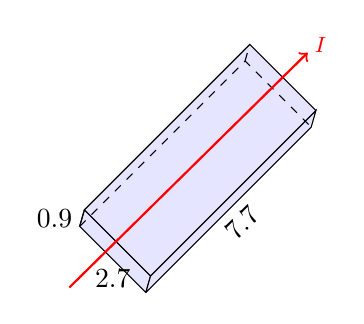
\begin{tikzpicture}[scale=1.5, x={(0.14cm,-0.14cm)},y={(0.04cm,0.14cm)},z={(-1.4cm,-1.4cm)}]
		\pgfmathsetmacro{\x}{4}
		\pgfmathsetmacro{\y}{1}
		\pgfmathsetmacro{\z}{1}
		\path (0,0,\y) coordinate (A) (\x,0,\y) coordinate (B) (\x,0,0) coordinate (C) (0,0,0)
		coordinate (D) (0,\z,\y) coordinate (E) (\x,\z,\y) coordinate (F) (\x,\z,0) coordinate (G)
		(0,\z,0) coordinate (H);
		\draw[fill=blue!10] (A)--(E)--(F)--(B);
		\draw[fill=blue!10] (A)-- node[below]{$2.7$} (B)-- node[below,sloped]{$7.7$} (C)--(G)--(F)--(B) (A)-- node[left]{$0.9$}(E)--(F)--(G)--(H)--(E);
		\draw [dashed,black] (A)--(D)--(C) (D)--(H);
		\draw[->, red, thick] (2, 1.3, 1.3)-- (2, 1, -0.15);
		\node[red] at (2, 1, -0.2) {\fontsize{8}{7} $I$};
		\end{tikzpicture}
	\end{center}



%  \begin{enumerate}
%    \item $R_\text{slab}= 5.7 \left(\frac{ 7.7 }{ 0.9\cdot 2.7 }\right) \Omega$
%    \item $R_\text{slab}= 5.7\Omega$
%    \item $R_\text{slab}= 5.7 \left(\frac{ 0.9 }{ 2.7\cdot 7.7 }\right)\Omega$
%    \item $R_\text{slab}= 5.7 \left(\frac{ 0.9 }{ 7.7 }\right)\Omega$
%    \item $R_\text{slab}= 5.7 \left(\frac{ 2.7 }{ 0.9\cdot 7.7 }\right)\Omega$
%  \end{enumerate}

\ans{This requires a substitution into the resistance formula: $R=\frac{\rho L}{A}$. Based on the fact that  we are told to use choice (B) from (a) selected above, we find that $R_\text{slab}= 5.7 \left(\frac{ 7.7 }{ 0.9 \cdot 2.7 }\right)\Omega$.}

\ans{
$R_\text{slab}= 5.7 \left(\frac{ 7.7 }{ 0.9 \cdot 2.7 }\right)\Omega$.
}

%Errors encoded into options (carry-over doable to implement, checks conceptual understanding of formula vs ability to read diagram.):
%  \begin{enumerate}
%      \item incorrect, corresponds to option (iii) above.
%      \item incorrect, leaves out a term in the formula
%      \item incorrect, option (ii) above.
%      \item correct, corresponds to option (i) above.
%      \item conflates resistance and resistivity, not understanding the significance of the dimension.
%  \end{enumerate}
%
%Randomization options: Values can be randomized easily.

\vspace{3mm}

\item (4 points) You are experimenting with various circuit configurations involving the slab and a voltage source. 2 dimensions are labeled (in red), and the 3rd is the one going "into" the page (not to scale). Which of the following configurations leads to the \textit{minimum} power dissipation by the slab?
  \begin{enumerate}
  	\begin{multicols}{2}
    \item\begin{minipage}{0.4\linewidth}
      \begin{center}
        \begin{circuitikz}
          \draw[american voltages]
          (0, 0) to[V<=$V_S$, invert] (0, 2) to (1, 2) to[short, white] (3, 2) to (4, 2) to[R, a=$10 \si{\ohm}$] (4, 0) to (0, 0);
          \filldraw [fill=blue!10, draw=black] (1,1.8) rectangle (3, 2.2);
          \node[red] at (2, 2.35) {\fontsize{8}{7} $7.7$};
          \node[red] at (0.75, 1.9) {\fontsize{8}{7} $0.9$};
          \draw (0,0) node[ground]{};
        \end{circuitikz}
      \end{center}
    \end{minipage}

    \item\begin{minipage}{0.4\linewidth}
      \begin{center}
        \begin{circuitikz}
          \draw[american voltages]
          (0, 0) to[V<=$V_S$, invert] (0, 2) to (1, 2) to[short, white] (3, 2) to (4, 2) to (4, 0) to (0, 0);
          \filldraw [fill=blue!10, draw=black] (1.5,1.8) rectangle (2.5, 2.2);
          \node[red] at (2, 2.35) {\fontsize{8}{7} $2.7$};
          \node[red] at (1.25, 1.9) {\fontsize{8}{7} $0.9$};
          \draw (0,0) node[ground]{};
        \end{circuitikz}
      \end{center}
    \end{minipage}
    \end{multicols}
    
	\begin{multicols}{2}
    \item\begin{minipage}{0.4\linewidth}
      \begin{center}
        \begin{circuitikz}
          \draw[american voltages]
          (0, 0) to[V<=$V_S$, invert] (0, 2) to (1, 2) to[short, white] (3, 2) to (4, 2) to (4, 0) to (0, 0);
          \filldraw [fill=blue!10, draw=black] (1,1.8) rectangle (3, 2.2);
          \node[red] at (2, 2.35) {\fontsize{8}{7} $7.7$};
          \node[red] at (0.75, 1.9) {\fontsize{8}{7} $0.9$};
          \draw (0,0) node[ground]{};
        \end{circuitikz}
      \end{center}
    \end{minipage}

    \item\begin{minipage}{0.4\linewidth}
      \begin{center}
        \begin{circuitikz}
          \draw[american voltages]
          (0, 0) to[V<=$V_S$, invert] (0, 2) to (1, 2) to[short, white] (3, 2) to (4, 2) to (4, 0) to (0, 0);
          \draw[american voltages]
          (0.5, 2) to (0.5, 1.4) to[R, a=$15 \si{\kilo\ohm}$] (3.5, 1.4) to (3.5, 2) to (4, 2) to (4, 0) to (0, 0);
          \filldraw [fill=blue!10, draw=black] (1.5,1.8) rectangle (2.5, 2.2);
          \node[red] at (2, 2.35) {\fontsize{8}{7} $2.7$};
          \node[red] at (1.25, 1.9) {\fontsize{8}{7} $0.9$};
          \draw (0,0) node[ground]{};
        \end{circuitikz}
      \end{center}
    \end{minipage}
    \end{multicols}

	\vspace{0.3cm}
    \item More than one of the labeled circuits has the same power dissipated across the slab.

  \end{enumerate}

\ans{The formula for power for a resistive element is $P=IV = \frac{V^2}{R}$. To minimize power, we want to maximize the resistance and minimize the voltage drop across the slab. For resistance, given that one of the cross-sectional area terms is $0.9\si{\centi\meter}$ in all given circuits, if we want greater resistance, we want current to flow in the direction of $7.7\si{\centi\meter}$, such that we see $7.7\si{\centi\meter}$ as the second-labeled dimension.

Next, for voltage drop; when the slab is the only element in the circuit apart from the voltage source as shown in (C), it necessarily has a $V_S$ volt drop across it. Adding a resistor in series decreases the voltage dropped across the slab, so power dissipation in the slab is the least in option (A).
}

\ans{(A)}

%Errors encoded into options:
%  \begin{enumerate}
%      \item on right track with regards to resistance, either misses (iii) or doesn't understand that power dissipation decreases with added series resistance.
%      \item doesn't interpret diagram correctly or doesn't read the question carefully (perhaps thinks the 2 dimensions labeled are the ones creating the cross-sectional area though the direction of current flow is clearly parallel to c).
%      \item The series resistance contributes a decrcease in power, though small.
%      \item similar to (ii), resistor in parallel forms independent KVL loop.
%      \item wrong, (iii) is optimal.
%  \end{enumerate}
%
%Randomization options: The values can be randomized easily.

\vspace{3mm}

\item Suppose you selected configuration (A) from above, which may or may not be correct. What is the power dissipated by the slab in that configuration?

%\begin{multicols}{2}
%\begin{enumerate}
%  \item $\frac{\left(V_S \cdot \frac{\frac{ 5.7 \cdot 2.7 }{ 0.9 \cdot 7.7 }}{\frac{ 5.7 \cdot 2.7 }{ 0.9 \cdot 7.7 } + 10 }\right)^2}{\frac{ 5.7 \cdot 2.7 }{ 0.9 \cdot 7.7 } \Omega}$
%  \item $\frac{\left(V_S \cdot \frac{\frac{ 5.7 \cdot 7.7 }{ 0.9 \cdot 2.7 }}{\frac{ 5.7 \cdot 7.7 }{ 0.9 \cdot 2.7 } + 10 }\right)^2 }{\frac{ 5.7 \cdot 7.7 }{ 0.9 \cdot 2.7 } \Omega}$
%  \item $\frac{V_S^2 \cdot 0.9 \cdot 2.7 }{ 5.7 \cdot 7.7 \Omega}$
%  \item $\frac{V_S^2 \cdot 0.9 \cdot 7.7 }{ 5.7 \cdot 2.7 \Omega}$
%  \item $\frac{V_S^2}{\frac{ 5.7 \cdot 7.7 }{ 0.9 \cdot 2.7 }\Omega + 10 \si{\ohm}}$
%\end{enumerate}
%\end{multicols}

\ans{Knowing that $P=\frac{V^2}{R}$, we can plug in directly, using $a \cdot b$ as the area and $c$ as the length. We account for the voltage divider on the series resistance; the voltage drop across the slab is $V_S \cdot \frac{\frac{ 5.7 \cdot 7.7 }{ 0.9 \cdot 2.7 }}{\frac{ 5.7 \cdot 7.7 }{ 0.9 \cdot 2.7 } + 10}$. The resulting answer is $P=\frac{V^2}{R}=\frac{\left(V_S \cdot \frac{\frac{ 5.7 \cdot 7.7 }{ 0.9 \cdot 2.7 }}{\frac{ 5.7 \cdot 7.7 }{ 0.9 \cdot 2.7 } + 10 }\right)^2 }{\frac{ 5.7 \cdot 7.7 }{ 0.9 \cdot 2.7 } \Omega}$.
}

\ans{$\frac{\left(V_S \cdot \frac{\frac{ 5.7 \cdot 7.7 }{ 0.9 \cdot 2.7 }}{\frac{ 5.7 \cdot 7.7 }{ 0.9 \cdot 2.7 } + 10 }\right)^2 }{\frac{ 5.7 \cdot 7.7 }{ 0.9 \cdot 2.7 } \Omega}$}

%Errors encoded into options:
%  \begin{enumerate}
%      \item doesn't get previous question and picks choice with just slab (but correct slab)
%      \item doesn't get previous question and picks choice with just slab (and wrong slab)
%      \item oversimplifies contribution of series resistance.
%      \item correct reasoning but wrong dimensions
%      \item correct
%  \end{enumerate}
%
%Randomization options: Numbers can be randomized.

%\newpage
%
%\item Now suppose you create configuration (B) from part (c), with power consumption $P_{\text{slab}}$. However, there are some size constraints now; given the choice to half the value of the voltage source ($V_S \rightarrow \frac{V_S}{2}$) \textit{or} double dimensions $a$ and $b$, leaving $c$ unchanged ($a \rightarrow 2a$, $b \rightarrow 2b$, $c$ same), which option minimizes power consumption more, and what is the new power after you make \textit{only this} change in terms of the old power?
%
%\begin{enumerate}
%  \item Halving the supply voltage; $P_{\text{slab}} \rightarrow \frac{P_{\text{slab}}}{4}$
%  \item Halving the supply voltage; $P_{\text{slab}} \rightarrow \frac{P_{\text{slab}}}{2}$
%  \item Doubling both $a$ and $b$ dimensions; $P_{\text{slab}} \rightarrow \frac{P_{\text{slab}}}{4}$
%  \item Doubling both $a$ and $b$ dimensions; $P_{\text{slab}} \rightarrow P_{\text{slab}}$ but the other change actually increases $P$.
%  \item They have identical effects on power minimization; $P_{\text{slab}} \rightarrow \frac{P_{\text{slab}}}{4}$
%\end{enumerate}
%
%\ans{Using $P=IV\equiv\frac{V^2}{R}\equiv I^2 R$; halving supply voltage will cut the power dissipated in 4, since the slab is the only circuit element and if $V_S$ becomes $\frac{V_S}{2}$, the power becomes $\frac{P_{\text{slab}}}{4}$. If $a$ and $b$ are both doubles, then the resistance stays the exact same since both length and area are doubled. From here, we recognize that halving the supply voltage is better, and we also calculated the power drop; we select choice (i).
%
%Errors encoded into options:
%  \begin{enumerate}
%      \item correct
%      \item selects correct high-level change but doesn't correctly apply effect of voltage change to power for a resistive element.
%      \item incorrect high-level change, might not read the dimension labels carefully, so they think that the doubling leads to area becoming 4x larger.
%      \item incorrect high-level change, correct reasoning but incorrect comparison
%      \item correct for supply voltage drop but arrives at same value for dimension doubling, similar error to (iii).
%  \end{enumerate}
%
%Randomization options: Numbers and ratios for various things (dimension change factors and voltage multiplication factors) can be randomized.
%}

\newpage

\item You realize that you can turn the slab into a variable resistor! You attach an ideal metal connector (shown in red) between one end of the resistive slab and some point in the middle of the slab, as shown below. 

\begin{figure}[h!]
  \begin{center}
      \begin{circuitikz}
        \draw[american voltages]
        (0, 0) to[V<=$V_S$, invert] (0, 2) to (1, 2) to[short, white] (3, 2) to (4, 2) to (4, 0) to (0, 0);
        \draw[american voltages, red,  thick]
        (3.5, 2) to (3.5, 0.9) to (2.4, 0.9) to (2.4, 1.8);
        \draw[american voltages, ->, red,  thick]
        (2.4, 0.9) to (2.4, 1.8);
        \filldraw [fill=blue!10, draw=black] (1,1.8) rectangle (3, 2.2);
        \draw[<->, thick, blue] (1, 1.4) to (2.4, 1.4);
        \draw[<->, thick, blue] (2.4, 1.4) to (3, 1.4);
        \node[blue] at (1.7, 1.2) {\fontsize{8}{7} $0.6$};
        \node[blue] at (2.7, 1.2) {\fontsize{8}{7} $2.1$};
        \node[red] at (2, 2.35) {\fontsize{8}{7} $2.7$};
        \node[red] at (0.75, 1.9) {\fontsize{8}{7} $0.9$};
        \draw (0,0) node[ground]{};
      \end{circuitikz}
    \end{center}
\end{figure}

Draw the equivalent circuit diagram for this physical configuration.

%\begin{enumerate}
%	
%	\begin{multicols}{2}
%  \item \hspace{0.1cm}
%  \begin{minipage}{0.5\linewidth}
%      \begin{center}
%            \begin{circuitikz}
%                  \draw[american voltages]
%                  (0, 0) to[V<=$V_S$, invert] (0, 2) to (1.5, 2) to[R=$\frac{ 5.7\cdot 2.7 }{ 0.9 \cdot 7.7 }\si{\ohm}$] (3, 2) to (4.5, 2) to (4.5, 0) to (0, 0);
%                  \draw (0,0) node[ground]{};
%            \end{circuitikz}
%      \end{center}      
%  \end{minipage}
%
%  \item  \hspace{0.1cm}
%  \begin{minipage}{0.5\linewidth}
%      \begin{center}
%            \begin{circuitikz}
%                  \draw[american voltages]
%                  (0, 0) to[V<=$V_S$, invert] (0, 2) to (1.5, 2) to[R=$\frac{ 5.7\cdot 2.1 }{ 0.9 \cdot 7.7 }\si{\ohm}$] (3, 2) to (4.5, 2) to (4.5, 0) to (0, 0);
%                  \draw (0,0) node[ground]{};
%            \end{circuitikz}
%            \end{center}
%  \end{minipage}
%  
%  
%  \end{multicols}
%  \vspace{0.5cm}
%  \begin{multicols}{2}
%
%
%  \item \hspace{0.1cm}
%  \begin{minipage}{0.5\linewidth}   
%      \begin{center}
%        \begin{circuitikz}
%          \draw[american voltages]
%          (0, 0) to[V<=$V_S$, invert] (0, 2) to (0.5, 2) to[R=$\frac{ 5.7\cdot 0.6 }{ 0.9 \cdot 7.7 }\si{\ohm}$] (2, 2) to[R=$\frac{ 5.7\cdot 2.1 }{ 0.9 \cdot 7.7 }\si{\ohm}$] (4, 2) to (4.5, 2) to (4.5, 0) to (0, 0);
%          \draw[american voltages]
%          (4.25, 2) to (4.25, 1.2) to (2, 1.2) to (2, 2);
%          \draw (0,0) node[ground]{};
%        \end{circuitikz}
%      \end{center}
%  \end{minipage}
%
%  \item \hspace{0.1cm}
%  \begin{minipage}{0.5\linewidth}
%      \begin{center}
%            \begin{circuitikz}
%                  \draw[american voltages]
%                  (0, 0) to[V<=$V_S$, invert] (0, 2) to (0.5, 2) to[R=$\frac{ 5.7\cdot 0.6 }{ 0.9 \cdot 7.7 }\si{\ohm}$] (2, 2) to[R=$\frac{ 5.7\cdot 2.1 }{ 0.9 \cdot 7.7 }\si{\ohm}$] (4, 2) to (4.5, 2) to (4.5, 0) to (0, 0);
%                  \draw[american voltages]
%                  (4.25, 2) to (4.25, 1.2) to[R=$\frac{ 5.7\cdot 2.1 }{ 0.9 \cdot 7.7 }\si{\ohm}$] (2, 1.2) to (2, 2);
%                  \draw (0,0) node[ground]{};
%            \end{circuitikz}
%      \end{center}
%  \end{minipage}
%  
%  
%\end{multicols}
%\vspace{0.5cm}
%
%  \item
%
%  None of these are equivalent to the physical configuration.
%
%\end{enumerate}


\ans{Recognizing that the red metal connection acts as a short, dividing the slab into "effective" and "ineffective" components, we can model the connection as an ideal short, and the original resistor is cut into 2 portions.

\begin{minipage}{0.5\linewidth}   
      \begin{center}
        \begin{circuitikz}
          \draw[american voltages]
          (0, 0) to[V<=$V_S$, invert] (0, 2) to (0.5, 2) to[R=$\frac{ 5.7\cdot 0.6 }{ 0.9 \cdot 7.7 }\si{\ohm}$] (2, 2) to[R=$\frac{ 5.7\cdot 2.1 }{ 0.9 \cdot 7.7 }\si{\ohm}$] (4, 2) to (4.5, 2) to (4.5, 0) to (0, 0);
          \draw[american voltages]
          (4.25, 2) to (4.25, 1.2) to (2, 1.2) to (2, 2);
          \draw (0,0) node[ground]{};
        \end{circuitikz}
      \end{center}
  \end{minipage}
}

%Errors encoded into options:
%  \begin{enumerate}
%      \item correct
%      \item the right resistor is shorted, but does not physically become a short itself.
%      \item the metal connector is ideal, not itself a resistor.
%      \item misses the point of the metal connector and uses wrong configuration.
%      \item misses the point of the metal connector
%  \end{enumerate}
%
%Randomization options: The values can be mixed up, answwer choices as well, though this question is meant to be conceptual.

\ans{
\begin{minipage}{0.5\linewidth}   
      \begin{center}
        \begin{circuitikz}
          \draw[american voltages]
          (0, 0) to[V<=$V_S$, invert] (0, 2) to (0.5, 2) to[R=$\frac{ 5.7\cdot 0.6 }{ 0.9 \cdot 7.7 }\si{\ohm}$] (2, 2) to[R=$\frac{ 5.7\cdot 2.1 }{ 0.9 \cdot 7.7 }\si{\ohm}$] (4, 2) to (4.5, 2) to (4.5, 0) to (0, 0);
          \draw[american voltages]
          (4.25, 2) to (4.25, 1.2) to (2, 1.2) to (2, 2);
          \draw (0,0) node[ground]{};
        \end{circuitikz}
      \end{center}
  \end{minipage}
}

% \item In a different slab-based configuration with a couple extra elements, we have the following circuit diagram. Select the option containing the image that is correctly labeled with currents and voltages, according to passive sign convention.

% \begin{figure}[h!]
%   \begin{center}
%       \begin{circuitikz}
%         \draw[american voltages]
%         (0, 0) to[V<=$V_S$, i=$I_S$, invert] (0, 3) to[R=$R_0$] (2, 3) to (2, 2) to[R=$R_1$] (6, 2) to (6, 3) to (7, 3) to (7, 0) to (0, 0);
%         \draw[american voltages]
%         (2, 3) to (2, 4) to[R=$R_2$] (4, 4) to[R=$R_3$] (6, 4) to (6, 3) to (7, 3) to (7, 0) to (0, 0);
%         \draw[american voltages]
%         (5.8, 4) to (5.8, 3.5) to (4, 3.5) to (4, 4);
%         \draw (0,0) node[ground]{};
%       \end{circuitikz}
%     \end{center}
%   \end{figure}

% \begin{enumerate}
%   \item

%   \begin{figure}[h!]
%   \begin{center}
%       \begin{circuitikz}
%         \draw[american voltages]
%         (0, 0) to[V<=$V_S$, i=$I_S$, invert] (0, 3) to[R=$R_0$, i=$I_{R_0}$] (2, 3) to (2, 2) to[R=$R_1$, i=$I_{R_1}$] (6, 2) to (6, 3) to (7, 3) to (7, 0) to (0, 0);
%         \draw[american voltages]
%         (2, 3) to (2, 4) to[R=$R_2$, i=$I_{R_2}$] (4, 4) to[R=$R_3$, i=$I_{R_3}$] (6, 4) to (6, 3) to (7, 3) to (7, 0) to (0, 0);
%         \draw[american voltages]
%         (5.9, 4) to (5.9, 3.1) to (4, 3.1) to (4, 4);
%         \draw[american voltages]
%         (0, 3) to[open, v_<=\phantom{x}$V_{R_0}$, invert] (2, 3);
%         \draw[american voltages]
%         (2, 2) to[open, v_<=\phantom{x}$V_{R_1}$, invert] (6, 2);
%         \draw[american voltages]
%         (2, 4) to[open, v_<=\phantom{x}$V_{R_2}$, invert] (4, 4);
%         \draw[american voltages]
%         (4, 4) to[open, v_<=\phantom{x}$V_{R_3}$, invert] (6, 4);
%         \draw (0,0) node[ground]{};
%       \end{circuitikz}
%     \end{center}
%   \end{figure}

%   \item

%   \begin{figure}[h!]
%   \begin{center}
%       \begin{circuitikz}
%         \draw[american voltages]
%         (0, 0) to[V<=$V_S$, i=$I_S$, invert] (0, 3) to[R=$R_0$, i=$I_{R_0}$] (2, 3) to (2, 2) to[R=$R_1$, i=$I_{R_1}$] (6, 2) to (6, 3) to (7, 3) to (7, 0) to (0, 0);
%         \draw[american voltages]
%         (2, 3) to (2, 4) to[R=$R_2$, i=$I_{R_2}$] (4, 4) to[R=$R_3$, i=$I_{R_3}$] (6, 4) to (6, 3) to (7, 3) to (7, 0) to (0, 0);
%         \draw[american voltages]
%         (5.9, 4) to (5.9, 3.1) to (4, 3.1) to (4, 4);
%         \draw[american voltages]
%         (0, 3) to[open, v_>=\phantom{x}$V_{R_0}$, invert] (2, 3);
%         \draw[american voltages]
%         (2, 2) to[open, v_>=\phantom{x}$V_{R_1}$, invert] (6, 2);
%         \draw[american voltages]
%         (2, 4) to[open, v_>=\phantom{x}$V_{R_2}$, invert] (4, 4);
%         \draw[american voltages]
%         (4, 4) to[open, v_>=\phantom{x}$V_{R_3}$, invert] (6, 4);
%         \draw (0,0) node[ground]{};
%       \end{circuitikz}
%     \end{center}
%   \end{figure}

%   \item

%   \begin{figure}[h!]
%   \begin{center}
%       \begin{circuitikz}
%         \draw[american voltages]
%         (0, 0) to[V<=$V_S$, i=$I_S$, invert] (0, 3) to[R=$R_0$, i=$I_{R_0}$] (2, 3) to (2, 2) to[R=$R_1$, i=$I_{R_1}$] (6, 2) to (6, 3) to (7, 3) to (7, 0) to (0, 0);
%         \draw[american voltages]
%         (2, 3) to (2, 4) to[R=$R_2$, i=$I_{R_2}$] (4, 4) to[R=$R_3$, i=$I_{R_3}$] (6, 4) to (6, 3) to (7, 3) to (7, 0) to (0, 0);
%         \draw[american voltages]
%         (5.9, 4) to (5.9, 3.1) to (4, 3.1) to (4, 4);
%         \draw[american voltages]
%         (0, 3) to[open, v_<=\phantom{x}$V_{R_0}$, invert] (2, 3);
%         \draw[american voltages]
%         (2, 2) to[open, v_>=\phantom{x}$V_{R_1}$, invert] (6, 2);
%         \draw[american voltages]
%         (2, 4) to[open, v_<=\phantom{x}$V_{R_2}$, invert] (4, 4);
%         \draw[american voltages]
%         (4, 4) to[open, v_<=\phantom{x}$V_{R_3}$, invert] (6, 4);
%         \draw (0,0) node[ground]{};
%       \end{circuitikz}
%     \end{center}
%   \end{figure}

%   \item

%   \begin{figure}[h!]
%   \begin{center}
%       \begin{circuitikz}
%         \draw[american voltages]
%         (0, 0) to[V<=$V_S$, i=$I_S$, invert] (0, 3) to[R=$R_0$, i=$I_{R_0}$] (2, 3) to (2, 2) to[R=$R_1$, i=$I_{R_1}$] (6, 2) to (6, 3) to (7, 3) to (7, 0) to (0, 0);
%         \draw[american voltages]
%         (2, 3) to (2, 4) to[R=$R_2$, i=$I_{R_2}$] (4, 4) to[R=$R_3$, i=$I_{R_3}$] (6, 4) to (6, 3) to (7, 3) to (7, 0) to (0, 0);
%         \draw[american voltages]
%         (5.9, 4) to (5.9, 3.1) to (4, 3.1) to (4, 4);
%         \draw[american voltages]
%         (0, 3) to[open, v_<=\phantom{x}$V_{R_0}$, invert] (2, 3);
%         \draw[american voltages]
%         (2, 2) to[open, v_>=\phantom{x}$V_{R_1}$, invert] (6, 2);
%         \draw[american voltages]
%         (2, 4) to[open, v_>=\phantom{x}$V_{R_2}$, invert] (4, 4);
%         \draw[american voltages]
%         (4, 4) to[open, v_<=\phantom{x}$V_{R_3}$, invert] (6, 4);
%         \draw (0,0) node[ground]{};
%       \end{circuitikz}
%     \end{center}
%   \end{figure}

%   \item More than one of the other labelings is valid.

% \end{enumerate}

% \ans{Only option (ii) is correctly labeled for all elements; option (i) is entirely backwards, option (iii) is incorrect for all resistors except $R_1$, and option (iv) is only correct for $R_1$ and $R_2$. Clearly option (v) doesn't hold true.

% Errors encoded into options:
%   \begin{enumerate}[(i)]
%       \item backwards, has PSC fully incorrect
%       \item correct
%       \item honestly not too sure how to implement wrong answers for a question like this, selectively correct.
%       \item honestly not too sure how to implement wrong answers for a question like this, selectively correct.
%       \item honestly not too sure how to implement wrong answers for a question like this, selectively correct.
%   \end{enumerate}

% Randomization options: Unsure about reliable randomization techniques. Perhaps similar to mt2? This question is a bit tangential anyways in its connection to the rest, certainly can be removed if needed.
% }


\item You construct a new circuit using several resistive slabs, a variable resistor and a voltage source, for which the equivalent circuit diagram is shown below. Which resistor has \textbf{no} current passing through it, regardless of it's value? Which resistor has the \textbf{most} current passing through it, regardless of its value? 
\\
\textit{Note}: Assume $R_1$ - $R_4$ are finite positive value resistors (non-zero and non-infinite).

\begin{figure}[h!]
  \begin{center}
      \begin{circuitikz}
        \draw[american voltages]
        (0, 0) to[V<=$V_S$, i=$I_S$, invert] (0, 3) to[R=$R_1$] (2, 3) to (2, 2) to[R=$R_3$] (6, 2) to (6, 3) to (7, 3) to (7, 0) to (0, 0);
        \draw[american voltages]
        (2, 3) to (2, 4) to[R=$R_2$] (4, 4) to[R=$R_4$] (6, 4) to (6, 3) to (7, 3) to (7, 0) to (0, 0);
        \draw[american voltages]
        (5.8, 4) to (5.8, 3.5) to (4, 3.5) to (4, 4);
        \draw (0,0) node[ground]{};
      \end{circuitikz}
    \end{center}
  \end{figure}

%\begin{enumerate}[(A)]
%  \item no current: $R_1$; most current: $R_1$
%  \item no current: $R_2$; most current: $R_3$
%  \item no current: $R_2$; most current: $R_1$
%  \item no current: $R_4$; most current: $R_1$
%  \item no current: $R_4$; most current: $R_2$
%\end{enumerate}

\ans{Note that $R_4$ is shorted by the ideal metal connector, whereas none of the other resistors are. Also, $R_1$ has the most current through it. We find that: no current: $R_4$; most current: $R_1$.}

\ans{no current: $R_4$; most current: $R_1$}

%Error Encodings; this should be a simple question, incorrect answers could stem from not reading the question correctly or not understanding how a resistor can be shorted. Not much randomization except for resistor labelings.


% \item You want to use your variable resistor to control the intensity of a dimmable light bulb. The light bulb can be modeled as a constant load resistance, $R_L = 1 \si{\kilo\ohm}$, whose intensity varies based on the current passing it. You attach the light bulb in the following configuration:

% \begin{figure}[h!]
% 	\begin{center}
% 		\begin{circuitikz}
% 			\draw[american voltages]
% 			(0, 0) to[V<=$10$V, invert] (0, 2) to (1, 2) to[short, white] (3, 2) to (4, 2) to[R=$R_L$]  (4, 0) to (0, 0);
% 			\draw[american voltages, red,  thick]
% 			(3.5, 2) to (3.5, 0.9) to (2.4, 0.9) to (2.4, 1.8);
% 			\draw[american voltages, ->, red,  thick]
% 			(2.4, 0.9) to (2.4, 1.8);
% 			\filldraw [fill=blue!10, draw=black] (1,1.8) rectangle (3, 2.2);
% 			\draw[<->, thick, blue] (1, 1.6) to (3, 1.6);
% 			\draw[<->, thick, blue] (2.4, 1.4) to (3, 1.4);
% 			\node[blue] at (1.7, 1.4) {\fontsize{8}{7} $L_{\text{tot}}$};
% 			\node[blue] at (2.7, 1.2) {\fontsize{8}{7} $L_2$};
% 			\draw (0, 0) node[ground]{};
% 		\end{circuitikz}
% 	\end{center}
% \end{figure}
 
%  In order for the light to turn on, the voltage across $R_L$ must be at least $2.5$V, but no more than $7.5$V (otherwise, the bulb will burn out). What is the range of values of $L_2$ for which the light bulb is on but not burned out?\\
%   Express your answer as a function of $L_{\text{tot}}$ and assume that the full slab has a resistance of $R_\text{slab} = 3 \si{\kilo\ohm}$, (i.e. when $L_2 = 0, R_{slab} = 3$k).



% \begin{enumerate}[(A)]
%   \item $0.25L_{\text{tot}} \leq L_2 \leq 0.75L_{\text{tot}}$
%   \item $L_2 \geq \frac{8}{9} L_{\text{tot}}$
%   \item $L_2 \leq \frac{8}{9} L_{\text{tot}}$
%   \item $L_2 \leq \frac{1}{4} L_{\text{tot}}$
%   \item Any distance $0 \leq L_2 \leq L_{\text{tot}}$ suffices.
% \end{enumerate}

% \ans{We can solve this problem for arbitrary load resistance $x$ and slab resistance $y$, and plug in our values in the end. We first must recognize that the metal connector shorts out $\frac{L_2}{L_{\text{tot}}}$ of the slab, leaving only $\frac{L_{\text{tot}}-L_2}{L_{\text{tot}}}$ "active". We can then use the voltage divider equation and form a double inequality:
% \begin{equation*}
% 0.25V_S \leq V_S \cdot \frac{x}{x+y\cdot\frac{L-L_2}{L}} \leq 0.75V_S
% \end{equation*}

% Rearranging and solving:
% \begin{equation*}
% \frac{y-3x}{y} \leq \frac{L_2}{L} \leq \frac{3y-x}{3y}
% \end{equation*}

% Now we plug in our specific numbers and arrive at option (iii).

% Errors encoded into options:
%   \begin{enumerate}[(i)]
%       \item doesn't read question carefully
%       \item flips order of lengths, solved as though increasing $L_2$ increased active region of slab, instead of decreasing
%       \item correct
%       \item oversimplifies calculations.
%       \item incorrect calculation on high end
%   \end{enumerate}

% Randomization options: I included specific values for demonstration but as the solution shows, any arbitrary resistances can be solved for, but a loop should be made to generate values; assert that all resistances and lengths are positive.
% }

\end{enumerate}
